\documentclass{article}

\title{Rendering Translucent Objects using Subsurface Scattering}
\author{Jo\~{a}o Pedro Jorge \and Willem Frishert}
\date{29-01-2007}

\usepackage{subfigure}
\usepackage[pdftex]{graphicx}

\begin{document}
\maketitle

\section{Introduction}
The implemented project goal was to render translucent objects. Those kind of objects can be seen everywhere, and good examples include marble, alabaster, human skin, plants, cloth, jade and many more.
All of the mentioned objects materials have in common the fact that they are not completely opaque due to scattering of light inside of them - know as subsurface scattering. Subsurface scattering causes the diffusion of scattered light and the blurring of small details on the surface of the objects.
Several papers approached these phenomena through the simulation of subsurface scattering. The chosen paper XXX REF XXX was published on SIGGRAPH quite recently and that was the motif that lead to our decision on choosing it. The approach behind the paper extends the diffusion theory present in medical physics related to the measurements of the optical properties of highly scattering materials.


\subsection{BRDF's vs. BSSRDF's}

While the well known BRDF (Bidirectional Reflectance Distribution Function) relates the light incident angle at a certain point with the outgoing angle at that very same point, the BSSRDF (Bidirectional Surface Scattering Reflectance Distribution Function) generalizes that concept and assumes that light might leave the object on a different point on a surface different from the one who arrived at (see Figure \ref{bssrdf_brdf}).

\begin{figure}[hbtp]
  \begin{center}
	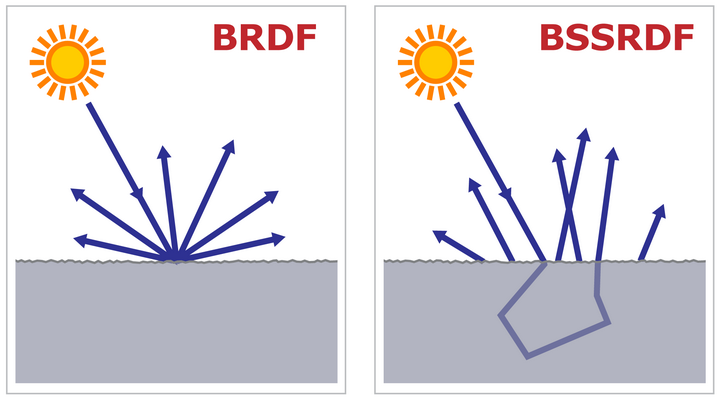
\includegraphics[scale=0.5]{./Pictures/BSSRDF_BRDF.png}
    \caption{BRDF vs BSSRDF Comparison}
    \label{bssrdf_brdf}
  \end{center}
\end{figure}

The BSSRDF, $S$, relates the outgoing radiance, $L _o(x _o, \vec{\omega} _o)$ at the point $x _o$ in the direction $\vec{x} _o$, to the incident flux, $\Phi _i(x _i, \vec{\omega} _i)$, at the point $x _i$ from direction $\vec{\omega} _i$:

\begin{equation}
dL _o(x _o, \vec{\omega} _o) = S(x _i, \vec{\omega} _i; x _o, \vec{\omega} _o) d\Phi _i(x _i, \vec{\omega} _i)
\end{equation}

Given a BSSRDF, the outgoing radiance is computed by integrating the incident radiance over incoming directions and area, $A$:

\begin{equation}
L _o(x _o, \vec{\omega} _o) = 
\int_{A}\int _{2\pi} S(x _i, \vec{\omega} _i; x _o, \vec{\omega} _o) L_i(x_i, \vec{\omega_i})(\vec{n} \cdotp \vec{\omega}_i) \,d\omega_i \,dA(x_i)
\end{equation}

\section{Model}
The BSSRDF model used to describe the translucency of a object consists of a sum of two scattering terms: a single scattering term and a diffusion approximation term.\cite{PracticalSSS} The latter term takes into account multiple scattering and is dominant.

\begin{equation}
S(x _i, \vec{\omega} _i; x _o, \vec{\omega} _o) =  {S}_{d}(x _i, \vec{\omega} _i; x _o, \vec{\omega} _o) + {S}^{(1)}(x _i, \vec{\omega} _i; x _o, \vec{\omega} _o)
\end{equation}

Originally, there are 4 parameters that influence the light transport when light hits the object surface and scatters. In \cite{HierarchicalSSS} this is reduced to two parameters: The reduced scattering coefficient ${\sigma}^{\prime}_s$ and the absorption coefficient $\sigma_{ a }$. 


\subsection{The Diffusion Approximation}
The diffusion approximation is based on the observation that light tends to become isotropic when multiple scattering occurs beneath the object surface. To approximate the contribution of the multiple scattering events, a dipole diffusion approximation is used. The dipole comes from medical physics and allows us to compute the radiant exitance for points on the surface.

\subsection{Two-Pass Technique for Evaluating the Diffusion Approximation}
In \cite{PracticalSSS} the diffuse approximation is computed in a single pass  which consumes a fair amount of time. To speed up the computation, Jensen et al. have improved their algorithm in \cite{HierarchicalSSS} by splitting it into a two pass rendering technique. The main idea is to decouple the computation of irradiance from the evaluation of the diffusion approximation. This allows the same irradiance values to be reused for different difussion approximation evaluations. Besides this, they also improve the efficiency for the evaluation of the diffusion approximation.

\subsubsection{Sampling the Irradiance}
To compute the irradiance on the surface, sample points have to be uniformly distributed over the object surface. The authors propose to use Turk's point repulsion algorithm which uses a relaxation method to spread out the sample points over the surface. The amount of sample points used depends on the surface total area and the mean free path $l_u$. The mean free path stands for the total distance a particle will travel inside the object before is it absorbed. Once the sample points are uniformly spread on the surface we can use global illumination techniques such as photon mapping or irradiance caching to obtain the irradiance at these particular points.

\subsubsection{Evaluating the Diffusion Approximation}
Can be used directly - heavy, lots of points; speak about the 3 options; hierarchical evaluation: best of both worlds; storage on the tree; subdivision criterion; computation of the radiant exitance and finally computing the Lo for each point.
input parameters: sigmas

\section{Implementation}
The implementation was initially divided into two parts: uniformly sampling the points and the hierarchical evaluation. However, the point sampling took much more time than it was expected and the work continued in that very same direction. It should be noticed that both of us knew the other one's part and the for several times we worked together in only one part.\linebreak
The code versioning and backup was done using Google Project Hosting SVN server\textbf{  XXX SHOULD WE PUT HERE THE LINK ???? XXX}. In this way the synchronization of the code made by both was easy, secure and straightforward.

\subsection{Renderer}
The initial proposal for a renderer mentioned a Pixar's RenderMan$^{\textregistered}$ compliant opensource renderer. The choice made was Pixie XXX Ref to it XXX. The framework seemed to be pretty stable and up-to-date. After several days studying RenderMan$^{\textregistered}$'s specification and trying to understand Pixie's implementation we decided that it was unrealistic to use it due to the lack of documentation and due to Renderman's low support for ray-tracing.\linebreak
The final choice for a renderer was then PBRT. The documentation was excellent and the renderer seemed to be widely used on the academic environment.\linebreak
\textbf{ XXX SHOULD WE TALK HERE ABOUT PBRT'S SET UP TIME ??? XXX }
Although PBRT is thought to be extended given its plugin nature, modelling a BSSRDF isn't that straightforward (as also mentioned myb the authors on the reference book). Several changes to its core must be made in order to get access to different information. The major changes are related with the {\it Shape, Material, GeometricPrimitive, Triangle and TriangleMesh} objects.

\subsection{First Pass - Sampling The Irradiance}
To obtain the irradiance at specific points on the objects surface, we used Turk's point repulsion algorithm. Firstly, we created triangle usesets and link them together so the triangles gain more knowledge about their neighbors. Then, in the second part, points are thrown on the triangle mesh and need to be roughly spread. We look a look at some different types of sampling methods and decided in the end to use a low discrepancy sampling method since it was best suited (See \ref{fig:turk_pointrepulsion_before}). Then, as Turk's algorithm mentions, we apply a relaxation technique which consist of two parts. Firstly, sample points compute how much force they exert on each other. In order to do this, the triangles, in which the points lay in, have to be transformed to become coplanar. The second part moves the points into the direction force. Either one of thee cases occurs when moving a point: it stays inside the triangle, it moves over the edge of a triangle onto another triangle or it moves over an edge where there is no neighboring triangle. For the last two cases, we used the knowledge provided by the usesets  to know what will happen to the point. Either it is moved on the edge of the triangle when there is no neighboring triangle or it is moved over the edge onto the new triangle. Mind that in the latter case, we need to rotate the point around the edge to make sure it falls in the triangle. Depending on initial set up of the points on the surface, the relaxation has to be iterated a number of times for the points to settle down. Using the low discrepancy sampling 5 iterators would be enough %(See \ref{fig:turk_pointrepulsion_after}). 
%\begin{figure}[htbp]
%  \begin{center}
%    \mbox{
%      \subfigure[before relaxation method] {\scalebox{0.3} %{\includegraphics[scale=0.5]{images/repulsion_before.png}}} \quad
%		\label{fig:turk_pointrepulsion_before}
%      \subfigure[[after relaxation method]   {\scalebox{0.3} %{\includegraphics[scale=0.5]{images/repulsion_after.png}}}
%		\label{fig:turk_pointrepulsion_after}
%      }
%    \caption{Applying Turk's point repulsion algorithm}
%    \label{fig:turk_pointrepulsion}
%  \end{center}
%\end{figure}

After the sample points have been uniformly spread, a basic Monte Carlo estimator can be used to calculate the irradiance. The estimator is given as:
\begin{equation}
I =  \frac{ \pi }{N } \sum_{i=1}^{ N}L_{sources} \left (  \Theta_i  \right )
\end{equation}

\subsection{Second Pass - Evaluating the Diffusion Approximation}

For the hierarchical evaluation, like the authors of the paper, we used an octree to store all our irradiance samples. In order to evaluate the total radiosity at a location $x$ on the surface of the object, the octree must be traversed starting from the root. For each voxel we test if:


\begin{figure}[tbh]
\centering
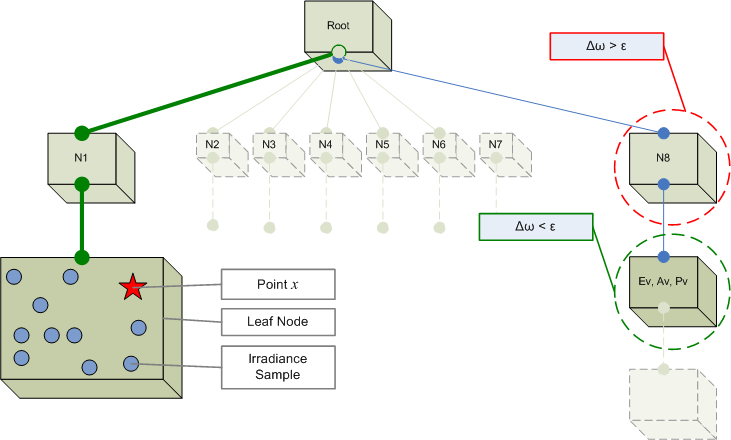
\includegraphics[scale=0.5]{./Pictures/Octree.png}
\caption{}
\label{Hierarchical Evaluation}
\end{figure}

octree - add and lookup; one or two schemes; the epsilon factor;

\section{Results}
\section{Conclusion}

% ### BIBLIOGRAPHY ###
\begin{thebibliography}{99}

\bibitem{HierarchicalSSS} H.W. Jensen and J. Buhler, 2002, A rapid hierarchical rendering technique for translucent materials. In {\it Proceedings of the 29th annual conference on Computer graphics and interactive techniques SIGGRAPH '02}, ACM Press pp. 576-581.

\bibitem{PracticalSSS} H.W. Jensen, S.R. Marschner, M. Levoy, and P. Hanrahan, 2001, A practical model for subsurface light transport. In {\it Proceedings of the 28th annual conference on Computer graphics and interactive techniques SIGGRAPH '01}, ACM Press pp. 63-69.

\end{thebibliography}


\end{document}
